% Substack header — v2.  Foreach-based reproduction of v1 (header.tex).
% Compile: ./build.sh header_v2.tex
%
% Spiral terminates at the true center (0,0).
% Knobs:
%   \rOuter        radius where line meets spiral
%   \turnsTotal    full turns of the spiral
%   \canvasEdge    outermost x of the horizontal line
%   \dotSpacing    cm between line dots         (controls line density)
%   \NdotsSpiral   dots on the spiral           (controls spiral density)
%   \dotRad        full dot radius              (line + first spiral dot)
%   \leftYSign     -1 = galaxy (180° rotation), +1 = yin-yang
%
% Spiral path: r(t) = rOuter*(1-t)²   — quadratic decay, reaches 0 at t=1
%              θ(t) = thetamax*t²     — smooth tangent at t=0 (joins line)
% Size fade:   ds   = dotRad*(1-t)    — linear; last dot has size 0 at origin

\documentclass[tikz,border=0pt]{standalone}
\usepackage{tikz}
\usepackage{xcolor}

% Palette
\definecolor{leftc}{HTML}{3F9580}     % green, teal-leaning
\definecolor{rightc}{HTML}{D43A28}    % burnt orange, red-leaning
\definecolor{bgc}{HTML}{FFF8E4}       % cream / parchment

\begin{document}
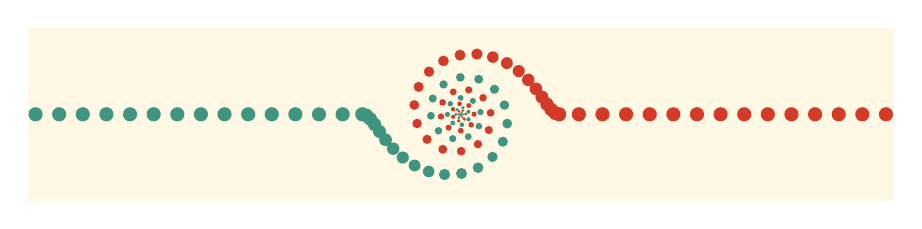
\begin{tikzpicture}[x=1cm,y=1cm]
  \useasboundingbox (-5.5,-1.1) rectangle (5.5,1.1);
  \fill[bgc] (-5.5,-1.1) rectangle (5.5,1.1);

  % ============================================================
  %                       PARAMETERS
  % ============================================================
  \def\rOuter{1.25}
  \def\turnsTotal{5.0}
  \def\canvasEdge{5.40}

  \def\dotSpacing{0.30}     % cm between line dots
  \def\NdotsSpiral{50}      % dots on the spiral
  \def\dotRad{0.09}

  \def\leftYSign{-1}

  % ============================================================
  %                       DERIVED
  % ============================================================
  \pgfmathsetmacro{\thetamaxDeg}{360*\turnsTotal}
  \pgfmathsetmacro{\lineLen}{\canvasEdge - \rOuter}
  \pgfmathtruncatemacro{\Nline}{\lineLen/\dotSpacing + 1}
  \pgfmathtruncatemacro{\NspiralMax}{\NdotsSpiral - 1}

  % ============================================================
  %                       RIGHT ARM (orange)
  % ============================================================
  \foreach \i in {1,...,\Nline} {
    \pgfmathsetmacro{\xx}{\canvasEdge - (\i-1)*\dotSpacing}
    \fill[rightc] (\xx, 0) circle (\dotRad cm);
  }
  \foreach \i in {0,...,\NspiralMax} {
    \pgfmathsetmacro{\tt}{\i/\NspiralMax}
    \pgfmathsetmacro{\onemt}{1-\tt}
    \pgfmathsetmacro{\rr}{\rOuter*\onemt*\onemt}
    \pgfmathsetmacro{\angd}{\thetamaxDeg*\tt*\tt}
    \pgfmathsetmacro{\ds}{\dotRad*\onemt}
    \fill[rightc] ({\rr*cos(\angd)}, {\rr*sin(\angd)}) circle (\ds cm);
  }

  % ============================================================
  %                       LEFT ARM (green) — mirrored
  % ============================================================
  \foreach \i in {1,...,\Nline} {
    \pgfmathsetmacro{\xx}{-\canvasEdge + (\i-1)*\dotSpacing}
    \fill[leftc] (\xx, 0) circle (\dotRad cm);
  }
  \foreach \i in {0,...,\NspiralMax} {
    \pgfmathsetmacro{\tt}{\i/\NspiralMax}
    \pgfmathsetmacro{\onemt}{1-\tt}
    \pgfmathsetmacro{\rr}{\rOuter*\onemt*\onemt}
    \pgfmathsetmacro{\angd}{\thetamaxDeg*\tt*\tt}
    \pgfmathsetmacro{\ds}{\dotRad*\onemt}
    \fill[leftc] ({-\rr*cos(\angd)}, {\leftYSign*\rr*sin(\angd)}) circle (\ds cm);
  }

\end{tikzpicture}
\end{document}
